This chapter introduces a new proof-of-concept framework called \textit{ILP(RL)}, a new learning framwork for RL problems using inductive learning with ILASP and planning with ASP.
The development of this framework is one of the main objectives of this project and we explain the framework in details in this Chapter.

\section{Overview}
\label{sec:overview}

\begin{figure}[!htb]
\centering
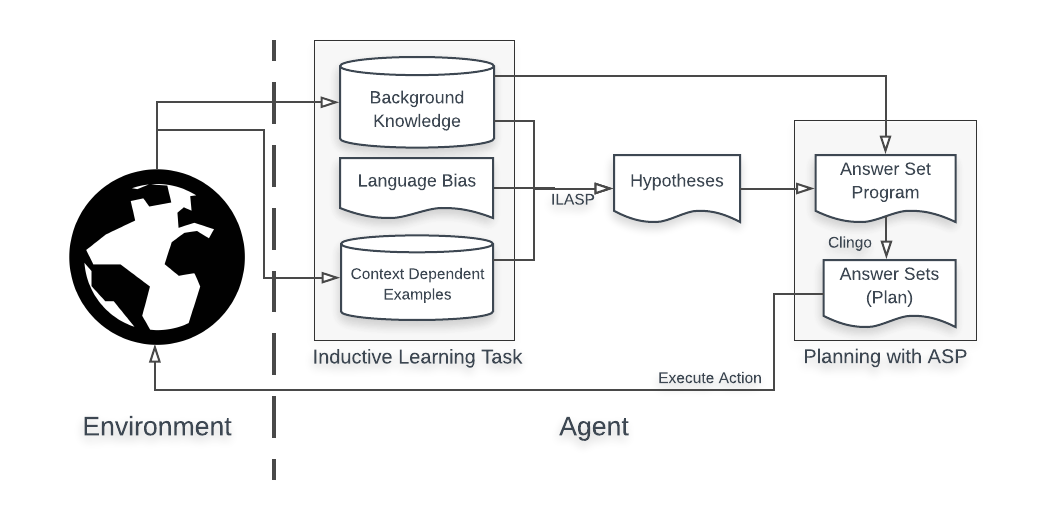
\includegraphics[width=1.0\textwidth]{./figures/architecture}
\caption{ILP(RL) overview}
\label{fig:ILPRL_overview}
\end{figure}

The overall architecture of ILP(RL), is shown in Figure \ref{fig:ILPRL_overview}. 
ILP(RL) mainly consists of two components: inductive learning with ILASP and planning with ASP. 

First step is inductive learning. An agent interacts with an unknown environment, 
and receives state transition experiences as context dependent examples. 
Together with pre-defined background knowledge and language bias, these examples are used to inductively learn and improve hypotheses, which are valid moves in the environment.

Second step is ASP planning. The interaction with the environment also gives the agent information about the environment, such as locations of walls or a goal. 
The agent remembers these information as background knowledge, and, 
together with the learnt hypotheses, uses it to make an action plan by solving an answer set program.
The plan is a sequence of actions and it navigates the agent in the environment.

The agent iteratively execute this cycle in order to learn and improve the hypotheses as well as an action planning. 
Mechanisms of each step are explained in details in the following sections.

\section{Environment}
\label{sec:environment}
Since there is no exisitng base framworks for ILP(RL), our focus on this project is to develop the preliminary version of the framework. 
Therefore, we use a very simple environmnet that allows us to see the potentials of our proposed architecture.
The base environment is a simple grid maze, and we assume that the environment is a discrete deterministic environment. 

We use an simple example to explain the environment as shown in Figure \ref{environment_example}.
States are expressed as X and Y coordinates. In Figure \ref{environment_example}, for example, the agent is located at \{X=2, Y=4\}.
The agent can take one of four possible actions at each time: up, down right and left.
Every time the agent takes an action, the agent receives the following experience: a reward R\textsubscript{t}, the next state S\textsubscript{t+1}, surrounding information of the current state.
The base environment mainly consists of three different elements: a goal, walls and paths.
The goal cell is the terminal state and the agent receives a positive reward when and the agent receives an negative rewards in any states except the terminal state.
When the agent reaches the terminal state, the agent receives a positive reward and the current episode is complete. 
Since the agent's goal is to maximise the total estimate rewards over time, this goal is equivalent to finding the shortest path from a starting state to a terminal state.

We also assume that, unlike an agent with other RL algorithms, the agent can see states of vertical and horizontal, but not diagonal, states around the agent. 
This assumption allows a agent to learn valid moves in the environment. For example, the agent at \{X=2, Y=4\} can see that there are walls at \{X=1, Y=4\} and \{X=2, Y=5\}.
More details of how to use these surrounding information is described in \ref{sec:inductive_learning_task}.

The applicability in more complex environment is not considered in this project and it is discussed in Further Research in Section \ref{sec:further_research}.

% The environment is provided outside of our algorithm,
\begin{figure}[!htb]
\centering
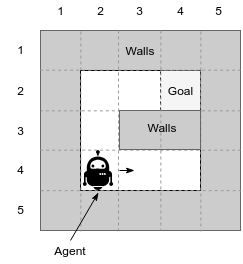
\includegraphics[width=0.4\textwidth]{./figures/environment_example}
\caption{5$\times$5 grid maze example}
\label{environment_example}
\end{figure}

\section{Inductive Learning Task}
\label{sec:inductive_learning_task}
The first step is constructing learning task using ILASP. The objective of the inductive learning is to learn valid moves in a given environment, which is used for generating action plan at the later step.
The definition of valid moves is as follows:

\begin{equation}
\begin{split}
&\textsf{state\_after(V1):-adjacent(right, V0, V1), state\_before(V1), action(right), wall(V0).}\\
&\textsf{state\_after(V0):-adjacent(right, V0, V1), state\_before(V1), action(right), not wall(V0).}\\
&\textsf{state\_after(V1):-adjacent(left, V0, V1), state\_before(V1), action(left), wall(V0).}\\
&\textsf{state\_after(V0):-adjacent(left, V0, V1), state\_before(V1), action(left), not wall(V0).}\\
&\textsf{state\_after(V1):-adjacent(down, V0, V1), state\_before(V1), action(down), wall(V0).}\\
&\textsf{state\_after(V0):-adjacent(down, V0, V1), state\_before(V1), action(down), not wall(V0).}\\
&\textsf{state\_after(V1):-adjacent(up, V0, V1), state\_before(V1),  action(up), wall(V0).}\\
&\textsf{state\_after(V0):-adjacent(up, V0, V1), state\_before(V1), action(up), not wall(V0).}
\end{split}
\label{target_hypothesis}
\end{equation}

where \textsf{state\_after} is the next state S\textsubscript{t+1}, \textsf{state\_before} is the current state S\textsubscript{t}. \textsf{action} is an action A\textsubscript{t} taken by the agent.
\textsf{adjacent(D, V0, V1)} specifies that V0 is next to V1 in the direction of D (e.g \textsf{adjacent(right, V0, V1)} means V0 is right next to V1). 
\textsf{wall(V)} and \textsf{not wall(V)} specify whether there is a wall or not wall in a state V respectively.
We describe the details of how to gain background knowledge, context dependent examples and language bias, necessary components for the agent to learn the above hypotheses.
The summary of a full ILASP learning task can be found in Appendix \ref{chap:learning_tasks}.
% Similar to other RL algorithms, an agent explores an environment by taking actions, which generates experiences. 
% These experiences need to be translated into ASP syntax and 
% and are recorded in as context dependent examples. 
% a positive example and background knowledge.
% Positive examples and background knowledge are used by ILASP for inductive learning, and background knowledge is used by both ILASP and ASP for solving for answer sets.

\subsection{Background Knowledge}
\label{subsec:background_knowledge}
First we define necessary background knowledge for inductive learning.
In order to learn a valid move for each direction in the form of state transition as shown in \ref{target_hypothesis}, we need to define the meaning of "being next to" a state.
This is defined as \textit{adjacent}, which is of the form:

\begin{equation} \label{eq:adjacent}
\begin{split}
&\textsf{adjacent(right, (X+1,Y),(X,Y)):-cell((X,Y)), cell((X+1,Y)).} \\
&\textsf{adjacent(left,(X,Y),  (X+1,Y)):-cell((X,Y)), cell((X+1,Y)).} \\
&\textsf{adjacent(down, (X,Y+1),(X,Y)):-cell((X,Y)), cell((X,Y+1)).} \\
&\textsf{adjacent(up,   (X,Y),  (X,Y+1)):-cell((X,Y)), cell((X,Y+1)).} \\
\end{split}
\end{equation}

where \textsf{cell} corresponds to a state, and \textsf{X} and \textsf{Y} represent coordinates respectively.
The rules \ref{eq:adjacent} are given as background knowledge and allow the agent to understand the relation of two adjacent states.
\textit{cell((X,Y))} is defined as follows:
\begin{equation} \label{eq:cell}
\begin{split}
    &\textsf{cell((0..X, 0..Y)).}
\end{split}
\end{equation}

where, 0..X defines the range of X coodinates and X and Y are the size of width and height of the environment respectively. 
For example, a grid maze shown in Figure\ref{environment_example} has a height and width of 5, thus the type cell is defined in the background knowledge as \textsf{cell((0..5, 0..5))}.

% While the agent explores the environment, it also keeps all the surrounding information as background knowledge,
% which will be stored in different repository, and are later used to generate a sequence of actions plan using H.

% This does not include state transition experience, as these state\_before and action takens are different at every timestep.
% In static environment (e.g no moving enermy), environment information remain the same across time, and thus it will be beneficial to remember.
% This principle is different from most RL methods, as they are model-free learning.
% In our simple maze environment, the agent is able to see the surrounding states and 
% these could be all wall position that the agent has seen so far, which can be
% wall((1, 5)). which represents the location of the wall.
% Another example could be a location of a teleportation if the agent sees it.
% These environment experiences are part of context examples in the positive examples.

\subsection{Context Dependent Examples}
Context dependent examples contain the results of the agent's interaction with an environment. Since all the interactions with the environment are examples of valid moves
they are used as positive examples. A positive example is expressed as a following ASP form:
\begin{equation}
\begin{split}
    \textsf{\#pos}(\{E\textsuperscript{inc}\}, \{E\textsuperscript{exc}\}, \textsf{\{C\}})
\end{split}
\end{equation}

It is equivalent to context-dependent partial interpretation (CDPI) in  $ILP_{LAS}^{context}$. 
As defined in the Equation \ref{eq:cdpi}, CDPI is of the form $\langle$ e, C $\rangle$ where e = $\langle$ E\textsuperscript{inc}, E\textsuperscript{exc} $\rangle$. 
Each of the components in CDPI is defined as follows:

\begin{defn}\label{def:ILPRL_context}
$C\textsubscript{ILP(RL)}$ contains an action a\textsubscript{t}, the current statestate s\textsuperscript{*}\textsubscript{t}, and adjacent walls of s\textsubscript{t}.
\label{def:context}
\end{defn}

\begin{defn} \label{def:ILPRL_inc}
$E\textsuperscript{inc}\textsubscript{ILP(RL)}$ includes s\textsubscript{t+1} $\in$ S such that:
\begin{itemize}
\item s\textsubscript{t+1} = s\textsuperscript{*}\textsubscript{t+1}
\item $ \forall A \in AS(B \cup H\textsubscript{t} \cup C\textsubscript{ILP(RL)})|$ s\textsubscript{t+1} $\not\in A$
\end{itemize}
\end{defn}

\begin{defn} \label{def:ILPRL_exc}
E\textsuperscript{exc}\textsubscript{ILP(RL)} includes S\textsubscript{t+1} $\in$ S such that:
\begin{itemize}
\item s\textsubscript{t+1} $\neq$ s\textsuperscript{*}\textsubscript{t+1}
\item $ \exists A \in AS(B \cup H\textsubscript{t} \cup C\textsubscript{ILP(RL)})|$ s\textsubscript{t+1} $\in A$
\end{itemize}
\end{defn}

where S\textsuperscript{*}\textsubscript{t+1} is the next state where the agent is at t+1, 
B is the background knowledge, H\textsubscript{t} is the hypotheses at t, 
S is all the states in the environment.

% Both e\textsuperscript{inc} and e\textsuperscript{exc} contain only the next state s\textsubscript{t+1}, expressed as \textit{state\_after((x,y))}, or empty.
% For context C, a\textsubscript{t} is translated int \textit{action((a))}, s\textsubscript{t} is translated into \textit{state\_before((x,y))}, and adjacent walls of s\textsubscript{t} are translated into \textit{wall((x$^\prime$,y$^\prime$))}.

In this report, we assume that part of context contains only whether a wall exists or not, with the presence of a wall, the agent cannot move to the state where a wall exist.

% \subsubsection{Positive examples in ASP syntax}
% \label{subsubsec:positive_examples_asp_syntax}

% For example, if the agent takes an action "up" to move from (1,1) to (1,2), all other states that the agent could have taken but did not are exclusions ((1,0), (1,1), (0,1) and (2,1) in this case).
% context examples include state\_before((X1,Y1)), which represents the position of the agent in x and y axis before an action is taken,
% action(A) is the action the agent has taken, and surrounding information, such as surrounding walls.

% Rewards are not used.
% (Discussed in details in Chapter XX).

% \textcolor{red}{There is no negative example as XXXX.}
% Using these positive examples, the agent is able to learn and improve hypothesis as it explore the environment and encounters new scenarios.
\begin{examp} \normalfont (Context dependent examples).

\begin{figure}[!htb]
\centering
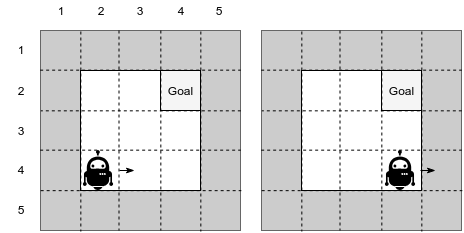
\includegraphics[width=0.7\textwidth]{./figures/pipeline_example1}
\caption{5$\times$5 grid maze example}
\label{example_pos_example}
\end{figure}

We use a simple 5x5 grid maze environment to highlight how an agent gains a positive example.
Suppose the agent does not know a hypothesis and takes an action "right" to move from (2,4) to (3,4) cell, as shown on the left in Figure \ref{example_pos_example}.
a\textsubscript{t} is "right" s\textsubscript{t} is (2,4) and s\textsubscript{t+1} is (3,4).
According to the Definition \ref{def:ILPRL_inc}, the answer sets of B $\cup$ H, does not cover s\textsubscript{t+1} since H = $\emptyset$, thus \textsf{state\_after((3,4))} is in e\textsuperscript{inc}.
All other alternative next states S\textsubscript{t+1} that the agent could have ended up by taking different actions
(down, up, and left) are in the exclusions.
Context includes a\textsubscript{t}, s\textsubscript{t} and S\textsubscript{neighbor} of walls.
The following positive example is generated.

\begin{equation}
\begin{split}
    \textsf{\#pos(} & \textsf{\{state\_after((3,4))\},}\\
                    & \textsf{\{state\_after((2,4)),state\_after((1,5)),state\_after((0,4)),state\_after((1,4))\},} \\
    & \textsf{\{state\_before((2,4)). action(right). wall((1, 4)). wall((4, 2)).\})}
\end{split}
\end{equation}

The next example illustrates a senario when the agent tries to move to a state where a wall is. 
The agent is at (4,4) and tries to move to a cell (5,4) by taking an action "right", as shown on the left in Figure \ref{example_pos_example}. 
In this case, however, there is a wall at (5,4) and therefore the agent cannot go to that cell.
Because of the blocking wall, s\textsubscript{t} and s\textsubscript{t+1} are (4,4).
The same the previous case, H = $\emptyset$ and therefore the answer sets of B $\cup$ H, does not cover s\textsubscript{t+1}.
All other alternative next adjacent states S\textsubscript{t+1} (4,3), (3,4), (5,4) and (4,5) are exclusions, and the context is collected.
From this example, the following positive example is generated:

\begin{equation}
\begin{split}
\textsf{\#pos(} & \textsf{\{state\_after((4,4))\}}, \\
                & \textsf{\{state\_after((4,3)),state\_after((3,4)),state\_after((5,4)),state\_after((4,5))\}} \\
                & \textsf{\{state\_before((4,4)). action(right). wall((5,4)). wall((4,5)).\}).}
\end{split}
\end{equation}

\end{examp}
\label{state_transition_example}

\subsection{Language Bias}
\label{subsec:language_bias}
We now define a search space using a language bias specified by \textit{mode declaration}.
As defined in \ref{def:las_context}, H $\subseteq$ S\textsubscript{M} for $ILP_{LAS}^{context}$, thus in order to learn the valid moves, S\textsubscript{M} is specified as follows:
\begin{equation} \label{eq:sm}
\begin{split}
&\textsf{\#modeh(state\_after(var(cell))).}\\
&\textsf{\#modeb(1, adjacent(const(action), var(cell), var(cell)), (positive)).} \\
&\textsf{\#modeb(1, state\_before(var(cell)), (positive)).} \\
&\textsf{\#modeb(1, action(const(action)),(positive)).} \\
&\textsf{\#modeb(1, wall(var(cell))).} \\
\end{split}
\end{equation}

where \textsf{\#modeh} and \textsf{\#modeb} are the \textit{normal head declarations} and the \textit{body declarations}. 
The first argument of each \textsf{\#modeb} specifies the maximum number of times that \textsf{\#modeb} can be used in each rule (also called \textit{recall}) \cite{Law2017}, 
which we specify 1 for all mode declarations in ILP(RL). \textsf{var(t)} is a placeholder for variable of \textit{type} \textsf{t}. In \ref{eq:sm}, we use \textsf{cell} for the variable type, which is grounded using on \textsf{cell} defined in \ref{eq:cell} in the background knowledge.
\textsf{const(t)} is a placeholder for constant term of type \textsf{t}, and type \textsf{t} must be specified as \textsf{\#constant(t, c)}, where \textsf{c} is a constant term., 
const(t) is specified as follows:

\begin{equation}
\begin{split}
&\textsf{\#constant(action, right).}\\
&\textsf{\#constant(action, left).}\\
&\textsf{\#constant(action, down).}\\
&\textsf{\#constant(action, up).}
\end{split}
\end{equation}

\textsf{action} type is specified as constant since ILASP needs to learn different hypothesis for each action, 
and can be found in each context dependent examples as specified in Definition \ref{def:context}.

\textsf{(positive)} in \textsf{\#modeb} specifies that the predicates only appear as positive and not negation as failure, which reduces the seach space. 
In ILP(RL), \textsf{wall(var(cell))} could appear as \textsf{not wall} in a hypothesis, and all other body declarations should only be positive due to the specification of \textsf{(positive)}. 

Finally, we define \textsf{\#max\_penalty} to specify the maximum size of the hypothesis. By default it is 15, however our target hypotheses defined in \ref{target_hypothesis} is larger than 15, and it is increased to 50.
Increasing \#max\_penalty allows ILASP to learn longer hypotheses at the expense of longer computation.
% For example, the search space in this particular setting is in XX.

\subsection{Hypothesis}
\label{sebsec:hypothesis}
Having defined the $ILP_{LAS}^{context}$ task T = $\langle$ B, S\textsubscript{M}, E\textsuperscript{+}, E\textsuperscript{-} $\rangle$, ILP(RL) is able to learn hypotheses H. 
Since B and S\textsubscript{M} are fixed, the hypotheses varies based on context dependent examples that the agent receives by interacting with an environment.
For example, in the early phase of ILP(RL) learning, the agent does not have many positive examples, and learns an hypothesis that is subset of the full target hypothesis that the agent can run in the environment.
ILP(RL) iteratively improves hypotheses as illustrated in Figure \ref{fig:ILPRL_overview}.

Formally,$ILP_{LAS}^{context}$ is executed by the following rule.
\begin{defn}\label{def:ILASP_run}
ILP(RL) runs $ILP_{LAS}^{context}$ to relearn H\textsubscript{new} if and only if $\forall$$\langle$ e, C$\rangle$ $\in$ E\textsuperscript{+}, $\exists$A $\in$ Answer Sets (B $\cup$ C $\cup$ H) such that A extends e
\end{defn}
where H is the current hypothesis that the agent has learnt so far. 
Learnt hypotheses are improved when a new positive example is added and the current hypothesis does not cover the new positive example.
If the current hypothese cover the new positive example, there is no need to re-execute ILASP.

The learnt hypothesis will be used to generate a plan, which we describe in the next section.

\begin{examp} \normalfont (Hypothesis).
Using the context dependent examples illustrated in Exaple \ref{example_pos_example}, we explain how the agent learns hypotheses.
Suppose that the agent takes an action "right" and gains one positive example, as shown on the right in Example \ref{example_pos_example}. 
The full learning task for this simple case is shown as follows:

\lstinputlisting[
  caption  = {Learning task example},
]{learning_task_example1.pl}
From the above learning task, ILASP learns the following hypothesis.
\begin{equation}
\begin{split}
\textsf{state\_after(V1) :- adjacent(left, V0, V1), state\_before(V0).}
\end{split}
\end{equation}

\lstinputlisting[
  caption  = {Additional context dependent example},
]{learning_task_example2.pl}

This hypothesis, for example, does not explain how to move "down". In order to learn how to move "down", it needs an positive example of moving up.
\end{examp}

\section{Planning with Answer Set Programming}
\label{sec:planning}

The learnt hypotheses using $ILP_{LAS}^{context}$ can be used to generate a sequence of action plan that the agent should follow.
In the following subsections, we explain how to create an answer set program and use the answer sets to make a plan in a maze environment.
\subsection{Answer Set Program}
\label{subsec:answer_set_program}
The ASP program should be constructed such that answer sets of ASP are a sequence of actions and states at each time step in ASP syntax. 

First, we use the learnt hypotheses by $ILP_{LAS}^{context}$ as part of the ASP program.
In the inductive learning phase in ILP(RL), we only need to differentiate between s\textsubscript{t} and s\textsubscript{t+1} as \textsf{state\_before} and \textsf{state\_after} respectively.
However, for the planning with ASP, the answer sets contains a sequence of actions and states for more than two time steps. 
In order to capture the notion of time sequences, we modify the ASP syntax by 
adding time \textit{T}. Specifically, the following mapping is required between ILASP and ASP planning syntax.

\begin{table}[H]
\centering
\begin{tabular}{|l|p{5cm}|p{5cm}|}
% \begin{tabular}{|l|l|p{1.5cm}|p{7cm}|l|l|l|l|}
\hline
No & ILASP syntax & ASP planning syntax\\ \hline
1 & \textsf{state\_before(V)} & \textsf{state\_at(V1, T)}  \\ \hline
2 & \textsf{state\_after(V)} & \textsf{state\_at(V1, T+1)}  \\ \hline
3 & \textsf{(empty body)} & \textsf{time(T)}  \\ \hline
4 & \textsf{action(A)} & \textsf{action(A, T)}  \\ \hline
\end{tabular}
\caption{ASP syntax mapping between }
\label{table:extension_specification}
\end{table}
The conversion from (empty body) to \textsf{time(T)} means that the body of all the hypotheses include \textsf{time(T)} in ASP planning syntax.
\begin{examp} \normalfont (Mapping of ASP syntax between $ILP_{LAS}^{context}$ and ASP).

\begin{equation}
\begin{split}
&\textsf{state\_after(V0) :- adjacent(right, V0, V1), state\_before(V1), action(right), not wall(V0).}\\
&\textsf{state\_after(V0) :- adjacent(left, V0, V1), state\_before(V1), action(left), not wall(V0).}\\
&\textsf{state\_after(V0) :- adjacent(down, V0, V1), state\_before(V1), action(down), not wall(V0).}\\
&\textsf{state\_after(V0) :- adjacent(up, V0, V1), state\_before(V1), action(up), not wall(V0).}
\end{split}
\end{equation}
The syntax of ASP is different from ILASP phase, because we need to include time sequence when solving ASP.
In ILASP, it is only state\_before and state\_after, but in plan generation, there will be more than one state transition.
These syntax conversion needs to be done for learnt hypothesis

\end{examp}

Second, we define a choice rule of actions, which is of the form:
\begin{equation}\label{eq:choice_rule}
\begin{split}
&\textsf{1\{action(down,T); action(up,T); action(right,T); action(left,T)\}1} \\
&\textsf{ :- time(T), not finished(T).}\\
\end{split}
\end{equation}

Action is given as a choice rule, and this choice rule states that action must be one of four actions: \textsf{down}, \textsf{up}, \textsf{right}, or \textsf{left}
at each time step T, as defined in the maximum and minimum integers 1.
The choice rules specify that one of four actions must be true unless \textsf{not finished(T)} or \textsf{time(T)} are satisfied, as defined in the body of the rule.
In RL scenarios, this means there is always action to be taken until the agent reaches a terminal state, 
When the agent reaches a terminal state, \textsf{finished(T)} is satisfied, otherwise time step T exceeds a maximum time steps allocated to the agent.

The maximum time steps are specified external and it is of the form:

\begin{equation}
\begin{split}
&\textsf{time(T\textsubscript{t}..T\textsubscript{max})}
\end{split}
\end{equation}
where T\textsubscript{t} is the current time step and T\textsubscript{max} is the maximum time steps.
For example, if an agent is at time step 0, and can take actions 100 times to find a goal time is defined as \textsf{time(0..100)}.

\textsf{finished(T)} determines whether the agent reaches the goal, which is defined in the following ASP form:

\begin{equation}\label{eq:asp_goal}
\begin{split}
&\textsf{finished(T):- goal(T2), time(T), T} \geq \textsf{T2.}\\
&\textsf{goal(T):- state\_at((X\textsubscript{goal}, Y\textsubscript{goal}), T), not finished(T-1).}\\
&\textsf{goalMet:- goal(T).}\\
&\textsf{:- not goalMet.}
\end{split}
\end{equation}

\textsf{state\_at((X\textsubscript{goal}, Y\textsubscript{goal}))} is the location of the goal, which is unknown to the agent in the beginning of the training.
The agent explores the environment until it finds the goal location.
In the other word, the agent cannot generate a plan to the goal untile the goal is found. 
Once the agent reaches the goal and \textsf{finished(T)} is satisfied, 
there will not be any actions at time T+1 since the body of the action choice rule defined in \ref{eq:choice_rule} is not satisfied.

Next, facts of walls information is provided as follows:
\begin{equation}
\begin{split}
&\textsf{wall((X,Y))}\\
\end{split}
\end{equation}

As defined in Definition \ref{def:ILPRL_context}, the agent is assumed to be able to see ajacent walls and used it as a context in positive examples in $ILP_{LAS}^{context}$. 
For ASP planning part, these wall information is accumulated as background knowledge as a separate repository, and used it for solving ASP. 

Next, the starting state for the planning provided as part of ASP. It is simply the current location of the agent where the actions plan is a starting point.
\begin{equation}
\begin{split}
\textsf{state\_at((X\textsubscript{start}, Y\textsubscript{start}), T)}
\end{split}
\end{equation}

In addition, the definition of ajacent and cell type are also provided, which are the same as what was defined as background knoweldge of $ILP_{LAS}^{context}$ (Equation \ref{eq:adjacent} and \ref{eq:cell})
ajacents.

Next, we need to incorporate a nortion of rewards in each state. Instead of maximising the total rewards, which is the objectives of most RL methods, 
we use optimisation statements as follow. 
\begin{equation}
\begin{split}
&\textsf{\#minimize\{1, X, T: action(X,T)\}}.
\end{split}
\end{equation}

The use of optimisation staetment is based on the assumption that the total rewards can be maximised by searching for optimal answer sets. 
While this works only subset of MDP, our preliminary research focuses on solving this particular MDP problem. 
    
Finally, we are only interested in a sequecne of actions and corresponding state as answer sets. 
Clingo can selectively include the atoms of certain predicates in the output and hide unselected ones. 
This is defined as follows:

\begin{equation}
\begin{split}
&\textsf{\#show state\_at/2.} \\
&\textsf{\#show action/2.}
\end{split}
\end{equation}

\begin{examp} \normalfont (Answer Set Program).

\begin{equation}
\begin{split}
&\textsf{state\_at((X\textsubscript{start}, Y\textsubscript{start}), T)}\\
&\textsf{\#minimize\{1, X, T: action(X,T)\}}.\\
&\textsf{\#show state\_at/2.} \\
&\textsf{\#show action/2.}\\
&\textsf{wall((X,Y))}
\end{split}
\end{equation}
\end{examp}

\subsection{Plan Execution}
\label{subsec:plan_execution}
Having defined the ASP, we explain the answer sets generated by the ASP and how to use the answer sets to execute the planning.

Since the rules \ref{eq:asp_goal} involves \textsf{state\_at((X\textsubscript{goal}, Y\textsubscript{goal})} and it is found only when the agent reaches the goal state, the plan generation is executed only after the agent finds the goal. 
Until the goal is found, the agent continues to explore the environment while impoving the hypotheses and collecting surrounding information.
Once the agent reaches the goal, the agent is told whether the state is a terminal state, and 
can generate a plan using the current hypotheses by solving Answer Set Program defined in \ref{subsec:answer_set_program}.

The output of the ASP is of the form:
\begin{equation}
\begin{split}
&\textsf{state\_at((x\textsubscript{t},y\textsubscript{t}),t), action(a\textsubscript{t},t),}\\
&\textsf{state\_at((x\textsubscript{t+1},y\textsubscript{t+1}),t+1), action(a\textsubscript{t+1},t+1),}\\
&\textsf{state\_at((x\textsubscript{t+2},y\textsubscript{t+2}),t+2), action(a\textsubscript{t+2},t+2),}\\
&\cdots\\
&\textsf{state\_at(((x\textsubscript{t+n},y\textsubscript{t+n}),t+n), action(a\textsubscript{t+n},t+n),}\\
&\textsf{state\_at((x\textsubscript{goal},y\textsubscript{goal}),t+n+1).} 
\end{split}
\end{equation}
% In RL algorithm, the agent also needs the positive reward by reaching a termination state. 

where \textit{n} is the number of time steps to take to reach the goal. 
\textit{action(A,T)} tells which action the agent should take at each time.
Given the answer set planning is correct, the agent follows the plan and reach the goal. 
The correctness of the planning is based on the correctness of the hypotheses as well as the wall surrounding information in the agent's background knowledge. 
For the correctness of the hypotheses, since the agent does not know all the information about the environment in the beginning of the learning,   
clingo might not generate correct sequence of actions leading to the goals.
Also if the agent has not seen enough surrounding walls, the plan of actions might be blocked by a wall that the agent has not seen. 

\begin{examp} \normalfont (Plan Execution).

Together with hypothesis, the background knowledge will used to solve for answer sets program. 
However, since hypothesis is not complete, there is more than one answer set at each time step. 
Since one of the answer sets state\_at is correct, the rest will be in the exclusions in the answer set, 
which is used to further improve the hypothesis in the next iteration of inductive learning.

In this example, the following is the answer set program

The answer set using the hypothesis XXX is 

XXX. 
The answer set using the improved hypothesis is XXX, 
Which correctly returns a sequence of actions and predicted states.

\end{examp}

This incorrect plan is also a source for learning a better hypothesis. 
As shown in Example XX, if the hypothesis is not a full hypotheses, outputs of ASP contain lots of \textsf{state\_at((X,Y), T)} at the same states. 
Given the agent is at one state at each time step, these duplicates are all included in exclusions, as defined in Definition \ref{def:ILPRL_exc}.

% When the agent encounters a new environment (e.g a new wall), this new information will be added to its background, which will be used to improved the hypothesis. 
% Similarly, after executing an action by following the generated plan, the agent receives a new positive example. If the new positive example is not covered by the current hypotheses, 
% ILASP reruns using the new example to improve the hypotheses. 
% next time ILASP gets executed.
% For example,
% \begin{equation*}
% \begin{split}
% &\textsf{state\_at((1,1),1), action(right,1)}\\
% &\textsf{state\_at((2,1),2), action(right,2)}\\
% &\textsf{state\_at((3,1),3), action(right,3)}\\
% &\textsf{state\_at((4,1),4), action(right,4)}\\
% &\textsf{state\_at((5,1),5)}, \cdots
% \end{split}
% \end{equation*}
% At the start of the learning, H is usually not correct or too general, using this H will generate lots of answer sets that are not useful for the planning.
% These examples will be collected and included as exclusions of a new positive example.

% This is formally defined in Algorithm.
% \begin{algorithm}
% \caption{ILP(RL)}\label{euclid}
% \begin{algorithmic}[1]
% \Procedure{ILP(RL) (B and E)}{}

% \While {True}
%     \State $\textit{H (inductive solutions)} \gets \text{run ILASP(T)}$
%     \State $\textit{plan(actions, states) answer sets} \gets \text{AS(B, H)}$
%     \While {actions in P}
%         \State $\textit{observed state} \gets \text{run clingo(T)}$
%         \If {$ \textit{observed state} \neq \textit{predicted state} $}
%             \State $\textit{H} \gets \text{run ILASP(T)}$
%             \EndIf
%         % \If {$ \textit{observed state not equal \textit{predicted state $}
%         % \EndIf
%     \EndWhile
%     % \If {$ new \ background \ encountered $}
%     %     % \State $\textit{H} \gets \text{run ILASP(T)}$
%     % \EndIf
%     % \For{i from 0 to N}
%     %     \If {$ A[i]\ is \ in \ T$}
%     %         \State \Return $FALSE$
%     %     \Else
%     %         \State Add A[i] to T
%     %     \EndIf
%     % \EndFor
% % \State \Return $TRUE$
% \EndWhile

% \EndProcedure
% \caption{ILP(RL) }
% \end{algorithmic}
% \end{algorithm}

% Everytime the agent executes an action by following the plan, it checks whether the observed state is that is expected.

% If there is a difference between the two, either

% B is incorrect

% H is not sophisticated enough,

% If that is the case, the agent runs ILASP again using more positive examples it collected during the plan execution.

\section{Exploration}
\label{exploration}
Exploration is one of the active research areas in RL, and is often discussed as a tradeoff between exploration and exploitation. 
While the agent exploit what is already learnt and follow the best policy and action selection so far.
It also needs to explore by taking a new action to discover a new state, which might make the agent discover an even shorter path and therefore higher total rewards in the future or in the long term. 
One of the most commonly used strategies is $\epsilon$-greedy strategy. 
As described in Chapter XXX, the agent takes an random action with a probability of $\epsilon$, which is a hiper-parameter.

ILP(RL) planning starts once the agent reaches a goal once. However it is likely that the agent has not seen all the environment
and therefore is likely to generates a sub-optimal plan. Therefore, similar to RL algorithms, the agent also has to explore a new state.

In our case, given the goal is found and the model is correct, it is likely that following the plan will maximize the total rewards, 
To avoid the agent from being stuck in a sub-optimal plan, the agent deliberately discards the plan and takes an random action with a probability of
epsilon (which is less than 1) TODO define this mathematically.

When the agent deviates from the planning, it discovers new information, which will be added to B.
Exploration is therefore necessary to make sure that the agent might discovers a shorter path than the current plan, which will be demonstrated in the experiment.

\begin{examp} \normalfont (Plan Generation).
Suppose the plan of the agent is the following. 

Suppose the agent decides to take an random action and moves "up", which may help it discover a new state. 
From the new state, the agent again plan to the goal from the current state. In this case, the new plan is 
Sub-optimal plan -> random exploration -> optimal policy.

\end{examp}
    
% Another common way is to decay the $\epsilon$ by the number of episodes, since at the beginning it is more likely that the agent has not fully explored the environment and therefore higher epsilon.

While statistical RL algorithms, such as Q-learning or Tile-coding explained in XX, update Q-value by a facter of alpha, 
ILP(RL) tends to strictly follow the plan the generated. Also it is known that model-based RL tends to get stuck in a sub-optimal if the model is incorrect, ILP(RL) also needs a exploration
And since the agent does not know when the perfect hypothesis in a particular environment is fully realised, it needs to keep exploring the environment even though

This strategy may not be appropriate in cases there safety is a priority (since it is random action.)

When the agent takes an random action and move into a new state, the agents creates a new plan from the new state and continue to move forward.

% Epsilon needs to be larger than Q-learnig because
It is simple to implement.

The reason for using random exploration is that it can be used for both benchmark and ILP(RL) and thus enables us to do a fair comparision between them.

After taking an random action, the agent again has a probably of epsilon for taking an random action. 
Throughout following the new plan, there is a small probalbility of chance that the agent takes an random action.

The current framework simply uses a simple random exploration, therefore even if the agent takes an random action and goes to a different state other than the planed one, 
the agent does the replan from the new state and quickly correct to the original plan path. 
This means it is likely that the agent of ILP(RL) only explores the adjacent cells and if there is a shorter path or new state
In other words, if the shorter path is far from the current state, the agent is unlikely be able to find the new state unless epsilon value is very high. 

\section{Implementation}
\label{Implementation}

% We use GVG-AI Framework for our experiments, which was created for the General Video Gamea AI Competition\footnote{http://www.gvgai.net/},
% a game environment for an agent that should be able to play a wide variety of games without knowing which games are to be played.
As shown in Figure \ref{fig:ILPRL_overview}, there are mainly three different components that need to be communicated: inductive learning with ILASP, planning with ASP and the external environment platform provided by VGDL with OpenAI interface.
All of them are communicated through the main driver written in Python. 
In the following section, part of low-level implementation of each part of the framework.

% \subsection{External Dependencies}

\subsection{Inductive Learning with ILASP}
We use ILASP2i, a inductive learning system developed in XX. 
ILASP2i is an interative version of ILASP2, and is designed to scale with the numbers of examples. 
ILASP2i also introduces the use of context dependent examples.
The latest ILASP officially available at the time of writing is ILASP3, which is designed to work on a noisy examples. 
Our positive examples do not contain noise, state transition positive examples, and ILASP2i was sufficient for our implemnetation.
which is discussed in Section XX. 
Alghough ILASP2i is designed to work with a large number of examples, inductive learning part is the bottleneck of our framework in terms of computational time. 
We did a number of optimisation in order to mitigate this. 

The first optimastion is the frequency of running ILASP. 
As already described in Definition \ref{def:ILASP_run}, ILASP is ran only if the current hypothesis does not cover all the examples accumulated so far.
Because of this, inductive learning takes place at the very early stage of learning, which is highlighted in the experiments in Chapter XX. 

The next optimisation is through the command line. 
ILASP2i has a number of options, and we explain each option using the actual command we use to run ILASP

% \begin{minted}[]
% ILASP --version=2i FILENAME.las -ml=8 -nc --clingo5 
% \end{minted}

\begin{lstlisting}[]
    ILASP --version=2i FILENAME.las -ml=8 -nc --clingo5 
    --clingo "clingo5 --opt-strat=usc,stratify" 
    --cached-ref=PATH --max-rule-length=8
\end{lstlisting}

where,
\begin{itemize}
\item \textsf{--version=2i} specifies that we use ILASP2i.
\item \textsf{--ml=8} specified the maximum numbers of body that each rule can have. The default length is 3.
\item \textsf{--nc} means no constrains, and omits constrains from the search space. Since our target hypothesis is not a constraint, this option recudes the search space.
\item \textsf{--clingo5} generates clingo 5 programs, which is fater, instead of clingo 4.3.
\item \textsf{--clingo "clingo5 --opt-strat=usc,stratify"} specifies clingo executable with the specified options. 
\textsf{usc, stratify} is unsatisfiable-core base optimisation with stratification using Gringo \cite{gringo}, a core XXX introduced in gringo version 3. REFERENCE.
\item \textsf{--cached-ref=PATH} enables the iterative mode, and keeps the output of the relevant example to a specified path, and start the learning from where it left before rather than going though all the examples.
\item \textsf{--max-rule-length=8} The default maximum number is 5.
\end{itemize}

Last optimisation is specifying search space.

Complexity. 

TODO the number of search space XX. 

\subsection{Planning with ASP}
Planning is computed using Clingo 5.

\begin{lstlisting}[]
    clingo5 --opt-strat=usc,stratify -n 0 FILENAME.lp
    --opt-mode=opt --outf=2
\end{lstlisting}

\begin{itemize}
\item \textsf{--clingo "clingo5 --opt-strat=usc,stratify"} specifies clingo executable with the specified options. 
\textsf{usc, stratify} is unsatisfiable-core base optimisation with stratification using Gringo \cite{gringo}, a core XXX introduced in gringo version 3. REFERENCE.
\item \textsf{-n 0} -n is an abbreviation of \textsf{models} to specify the maximum number of answer sets to be computed. \textsf{-n 0} means to compute all answer sets.
\item \textsf{--opt-mode=opt} computes optimal answer sets
\item \textsf{--outf=2} makes the output in JSON\footnote{http://json.org/} format
\end{itemize}

\subsection{Environment Platform}
\subsubsection{The Video Game Definition Language (VGDL)}

\begin{figure}[!ht!b]
\centering
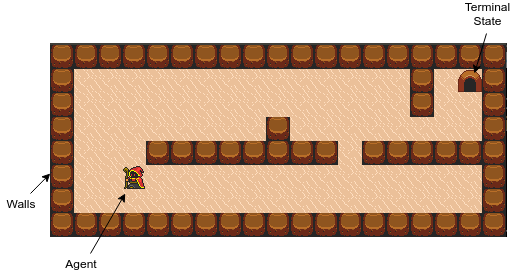
\includegraphics[width=1\textwidth]{./figures/env_sample}
\caption{The VGDL (Video Game Definition Language) environment example} 
\label{VGDL_sample}
\end{figure}

We use the Video Game Definition Language (VGDL), which is a high-level description language for 2D video games providing a platform for computational intelligence research (\cite{Schaul2013}).
The VGDL allows users to easily craft their own environments, which makes us possible to do various experiments without relying on a default environment. 
All objects in the games can be described as a sprite in the \textit{SpriteSet}, and users can define the objects' properties such as orientation or movements.
The representation of each object can be specified in \textit{LevelMapping} and allows users to customize an original map.
\textit{InteractionSet} specify the effects of objects when two objects interact in the game.
\textit{TerminationSet} specify the conditions for ending the game.
XX VDGL mapping example.

The VGDL platform provides an interface with OpenAI Gym (\cite{Brockman2016}), which is a commonly used benchmark platform.

The base game is a simple maze as shown in Figure \ref{VGDL_sample}.
There are 3 different types of cells: a goal cell, walls and paths. The agent can take 4 different actions: up, down, right and left.
The environment is not known to the agent in advance, and it attempts to find the goal by exploring the environment.
In all experiments, the agent receives -1 in any states except the goal state, where it gains a reward of 10.
Once the agent reaches the goal, or termination state, that episode is finished and the agent start the next episode from the starting point.

TODO write more details of how you make your own environment
We use PyVGDL\footnote{https://github.com/schaul/py-vgdl/}, which is a high-level VGDL on top of pygame\footnote{https://www.pygame.org}, 
a Python modules designed for writing video games.


We develop our framework ILP(RL) using an environment of VDGL game.

\subsubsection{OpenAI Gym}
The communication between VGDL environment and an agent, ILP(RL), is through OpenAI Gym, which is 
% The VDGL game is communicated with RL algorithms through OpenAI Gym. 

\lstinputlisting[
  language = Python,
  caption  = {OpenAI gym interface},
]{openai.py}

\begin{itemize}
\item \textsf{env.reset()} resets the game and the agent starts from the starting position. We call it when the agent starts a new episode.
\item \textsf{env.step(action)} returns an observation of taking an action, which include the state location of the agent in terms of x and y coodinates, reward of the state, an boolean value indicating whether the agent reaches an terminal state.
The action is chosen by an RL algorithm of your choice. In the case of ILP(RL), action is chosen by the ASP planning or random exploration strategy between 0 and 3.
\item \textsf{env.render()} renders one frame of the environment to see the movement of the agent in pygame.
\end{itemize}

\subsection{The Main Driver}
All of the above are connected in Python script.

The main roles of the driver is handling the communications between an environment and an agent as well as the communications within the agent.

\begin{description}
\item[Communication between an environment and an agent]

When an agent takes an action in a VDGL game environment, 
the output of the environment is returned by OpenAI gym environment, which is of the form:

This works the same for any RL algorithms when using OpenAI gym environment. 


subprocess

\item[Communication within the agent]

\end{description}
